\documentclass{beamer}
\usepackage[utf8]{inputenc}

\usepackage{fourier} %font utopia imported
\usetheme{Madrid}
\usecolortheme{default}

%------------------------------------------------------------
%This block of code defines the information to appear in the
%Title page
\title[Synthesizing OA in Maude] %optional
{Synthesizing Orchestration Algorithms of \\Complex Scenarios using Maude}
\date{\today}
\usepackage{booktabs}
\usepackage{natbib}
\usepackage{multicol}
\usepackage{listings}
\usepackage{environ}
\usepackage{graphicx}
\usepackage{amsfonts}
\usepackage{amsmath}
\usepackage{amssymb}
\usepackage{stmaryrd}
\usepackage{amstext}
\usepackage{semantic}
\usepackage{semantic}
\usepackage{algorithm}
\usepackage{algpseudocode}
\usepackage{etoolbox}
\usepackage{paralist}
\usepackage{verbatim}


\usepackage[capitalise,nameinlink]{cleveref}

% Comments

\newcommand{\simon}[1]{%
  {\scriptsize
      \textbf{\textcolor{red}{Simon: #1}}
  }%
}%

\newcommand{\peter}[1]{%
  {\scriptsize
      \textbf{\textcolor{blue}{Peter: #1}}
  }%
}%

% Paper specific notation

\setlength{\intextsep}{10pt}

\crefname{problem}{problem}{problems}

\newcommand{\inputV}{v}
\newcommand{\consistent}{\ensuremath{\mathit{Consistent}}}
\newcommand{\remaining}{\ensuremath{\mathit{Remaining}}}
\newcommand{\dontcare}{\_}
\newcommand{\defined}{\ensuremath{\mathit{defined}}}
\newcommand{\undefined}{\ensuremath{\mathit{undefined}}}
\newcommand{\properties}{P}
\newcommand{\satisfies}{\vDash}
\newcommand{\simulator}{\mathcal{A}}
\newcommand{\Induced}[2]{\llbracket #1 \rrbracket_{#2}}
\newcommand{\timebase}{\setreal_{\geq 0}}
\newcommand{\stepbase}{\setreal_{> 0}}
\newcommand{\variables}[1]{\mathit{VAR_{#1}}}
\newcommand{\stateset}[1]{S_{#1}}
\newcommand{\runstate}[1]{S^{R}_{#1}}
\newcommand{\state}[1]{s_{#1}}
\newcommand{\inputs}[1]{U_{#1}}
\newcommand{\parameters}[1]{P_{#1}}
\newcommand{\inputvar}[1]{u_{#1}}
\newcommand{\outputs}[1]{Y_{#1}}
\newcommand{\outputvar}[1]{y_{#1}}
\newcommand{\mayReject}{M}
\newcommand{\backtrack}{B}
\newcommand{\values}{\mathcal{V}}
\newcommand{\valuesExchanged}{\mathcal{V_{E}}}
\newcommand{\true}{\mathit{true}}
\newcommand{\false}{\mathit{false}}
\newcommand{\feedthrough}[1]{F_{#1}}
\newcommand{\reactivity}[1]{R_{#1}}
\newcommand{\fset}[1]{\mathtt{set}_{#1}}
\newcommand{\fget}[1]{\mathtt{get}_{#1}}
\newcommand{\fdoStep}[1]{\mathtt{step}_{#1}}
\newcommand{\fpreset}[1]{\mathtt{preSet}_{#1}}
\newcommand{\fpreget}[1]{\mathtt{preGet}_{#1}}
\newcommand{\fpredoStep}[1]{\mathtt{preStep}_{#1}}
\newcommand{\ftime}{\mathtt{ftime}}
\newcommand{\maxStep}[1]{\mathtt{h}_{#1}}
\newcommand{\timestamp}[1]{\varphi(#1)}
\newcommand{\feedsto}[2]{U_{#1}^{#2}}
\newcommand{\CheckCon}{\mathit{CheckConv}}
\newcommand{\stepfound}{\mathit{Step\_found}}
\newcommand{\valuations}{\mathit{V}}
\newcommand{\valuation}{\mathit{v}}


\newcommand{\dom}[1]{\mathit{dom(#1)}}
\newcommand{\algebraic}[1]{\mathit{algebraic_{#1}}}

 

\newcommand{\precondition}{\mathit{Pre}}


\newcommand{\complexity}{Com}
\newcommand{\master}{\mathcal{A}}
\newcommand{\alloutputs}{Y}
\newcommand{\allfeedthroughs}{F}
\newcommand{\allreactivity}{R}
\newcommand{\alldelayed}{D}

\newcommand{\allcontracts}{\mathcal{C}}
\newcommand{\coupling}{L}
\newcommand{\allinputs}{U}
\newcommand{\fmus}{C}
\newcommand{\fmusLoop}{C_{loop}}
\newcommand{\sequence}[1]{\pargroup{#1}}
\newcommand{\functioncall}{f}
\newcommand{\initcall}{I}
\newcommand{\allfunctioncalls}{F}
\newcommand{\fmu}[1]{\texttt{#1}}
\newcommand{\signal}[1]{\texttt{#1}}
\newcommand{\before}[2]{\ensuremath{#1 \twoheadrightarrow #2}}
\newcommand{\ibefore}[2]{\ensuremath{#1 \rightarrow #2}}
\newcommand{\after}[1]{{#1}'}
\newcommand{\aftern}[2]{{#1}^{(#2)}}
\newcommand{\stateafter}[2]{\ensuremath{\state{#1}^{(#2)}}}
\newcommand{\minstep}{\ensuremath{h_{min}}}


\newcommand{\etime}{\ensuremath{E}}

\newcommand{\verifier}{\mathit{Verifier}}

\newcommand{\turnOn}{\mathit{TurnPreconditionsOn()}}
\newcommand{\turnOff}{\mathit{TurnPreconditionsOff()}}

\newtheorem{procedure}{Procedure}{}
\newtheorem{assumption}{Assumption}{}

\newtheorem{experiment}{Experiment}{}

\algrenewcommand\alglinenumber[1]{\scriptsize #1:}% Adapt size of line numbers in algorithm

\algnewcommand\algorithmicforeach{\textbf{for each}}
\algdef{S}[FOR]{ForEach}[1]{\algorithmicforeach\ #1\ \algorithmicdo}
% New definitions
\algnewcommand\algorithmicswitch{\textbf{switch}}
\algnewcommand\algorithmiccase{\textbf{case}}
\algnewcommand\algorithmicassert{\texttt{assert}}
\algnewcommand\Assert[1]{\State \algorithmicassert(#1)}%
% New "environments"
\algdef{SE}[SWITCH]{Switch}{EndSwitch}[1]{\algorithmicswitch\ #1\ \algorithmicdo}{\algorithmicend\ \algorithmicswitch}%
\algdef{SE}[CASE]{Case}{EndCase}[1]{\algorithmiccase\ #1}{\algorithmicend\ \algorithmiccase}%
\algtext*{EndSwitch}%
\algtext*{EndCase}%



% Generic stuff

\newcommand{\footurl}[1]{\footnote{\url{#1}}}

% Math
\newcommand{\brackets}[1]{\ensuremath{ \left[ #1 \right] }}
\newcommand{\tuple}[1]{\ensuremath{ \left\langle #1 \right\rangle }}
\newcommand{\set}[1]{\ensuremath{ \left\{ #1 \right\}}}
\newcommand{\system}[1]{\ensuremath{ \begin{cases} #1 \end{cases}}}
\newcommand{\rightgroup}[1]{\ensuremath{ \left. \begin{matrix} #1 \end{matrix} \right\} } }
\newcommand{\pargroup}[1]{\ensuremath{ \left( #1 \right)}}
\newcommand{\inv}[1]{\ensuremath{\pargroup{ #1 }^{-1}}}
\newcommand{\dert}[1]{\ensuremath{ \dot{#1} }}
\newcommand{\ddert}[1]{\ensuremath{ \ddot{#1} }}
\newcommand{\partialder}[2]{\ensuremath{ \frac{\partial#1}{\partial#2} }}
\newcommand{\setreal}[0]{\ensuremath{\mathbb{R}}}
%\newcommand{\setbool}[0]{\ensuremath{\mathit{Bool}}}
\newcommand{\setnat}[0]{\ensuremath{\mathbb{N}}}
\newcommand{\norm}[1]{\left\lVert#1\right\rVert}
\newcommand{\bnorm}[1]{\big\lVert#1\big\rVert}
\newcommand{\abs}[1]{\left|#1\right\|}
\newcommand{\xs}[2]{\ensuremath{#1^{\left[#2\right]}}}
\newcommand{\infinitynorm}[1]{\left\lVert#1\right\rVert_\infty}


\newcommand{\vectorOne}[1]{\brackets{%
\begin{matrix}
  #1
 \end{matrix}%
}}
\newcommand{\vectorTwo}[2]{\brackets{%
\begin{matrix}
  #1 \\
  #2
 \end{matrix}%
}}
\newcommand{\vectorThree}[3]{\brackets{%
\begin{matrix}
  #1 \\
  #2 \\
  #3
 \end{matrix}%
}}
\newcommand{\vectorFour}[4]{\brackets{%
\begin{matrix}
  #1 \\
  #2 \\
  #3 \\
  #4
 \end{matrix}%
}}
\newcommand{\vectorFive}[5]{\brackets{%
\begin{matrix}
  #1 \\
  #2 \\
  #3 \\
  #4 \\
  #5
 \end{matrix}%
}}
\newcommand{\vectorSix}[6]{\brackets{%
\begin{matrix}
  #1 \\
  #2 \\
  #3 \\
  #4 \\
  #5 \\
  #6
 \end{matrix}%
}}
\newcommand{\vectorSeven}[7]{\brackets{%
\begin{matrix}
  #1 \\
  #2 \\
  #3 \\
  #4 \\
  #5 \\
  #6 \\
  #7
 \end{matrix}%
}}
\newcommand{\vectorEight}[8]{\brackets{%
\begin{matrix}
  #1 \\
  #2 \\
  #3 \\
  #4 \\
  #5 \\
  #6 \\
  #7 \\
  #8
 \end{matrix}%
}}

\newenvironment{aligneq*}%
{
\begin{equation*}
\begin{aligned}
}{
\end{aligned}
\end{equation*}
}

\newenvironment{aligneq}%
{
\begin{equation}
\begin{aligned}
}{
\end{aligned}
\end{equation}
}



%enable \cref{...} and \Cref{...} instead of \ref: Type of reference included in the link
%Nice formats for \cref
\usepackage{iflang}
\IfLanguageName{ngerman}{
  \crefname{table}{Tab.}{Tab.}
  \Crefname{table}{Tabelle}{Tabellen}
  \crefname{figure}{\figurename}{\figurename}
  \Crefname{figure}{Abbildungen}{Abbildungen}
  \crefname{equation}{Gleichung}{Gleichungen}
  \Crefname{equation}{Gleichung}{Gleichungen}
  \crefname{listing}{\lstlistingname}{\lstlistingname}
  \Crefname{listing}{Listing}{Listings}
  \crefname{section}{Abschnitt}{Abschnitte}
  \Crefname{section}{Abschnitt}{Abschnitte}
  \crefname{paragraph}{Abschnitt}{Abschnitte}
  \Crefname{paragraph}{Abschnitt}{Abschnitte}
  \crefname{subparagraph}{Abschnitt}{Abschnitte}
  \Crefname{subparagraph}{Abschnitt}{Abschnitte}
}{
  \crefname{section}{Sect.}{Sect.}
  \Crefname{section}{Section}{Sections}
  \crefname{listing}{\lstlistingname}{\lstlistingname}
  \Crefname{listing}{Listing}{Listings}
}
\crefname{section}{Sect.}{Sect.}
\Crefname{section}{Section}{Sections}
\crefname{listing}{\lstlistingname}{\lstlistingname}
\Crefname{listing}{Listing}{Listings}

\crefname{assumption}{Assumption}{Assumptions}


% update later with official instructions from Springer
\def\orcidID#1{${}^{\smash{\href{https://orcid.org/#1}{\protect\raisebox{-1.25pt}{\protect
\includegraphics{images/orcid_color-eps-converted-to}}}}}$}




\urlstyle{same}
\author[Thrane, S.] % (optional)
{Simon Thrane Hansen \newline Ph.D. Student \newline Aarhus University}


\date[AU 2021] % (optional)
{\today}

%\logo{\includegraphics[height=1.5cm]{lion-logo.jpg}}

%End of title page configuration block
%------------------------------------------------------------



%------------------------------------------------------------
%The next block of commands puts the table of contents at the 
%beginning of each section and highlights the current section:


%------------------------------------------------------------
\begin{document}

%The next statement creates the title page.
\frame{\titlepage}

\begin{frame}{Overview}
    \tableofcontents
\end{frame}

\section{Recap Simple Scenarios}
\begin{frame}{Simulation of simple scenario}
    Last time we covered simple scenarios by describing the rules of the actions that formed the step operation graph - that for simple scenarios only contain trivial SCC.
    \begin{columns}[T] % align columns
        \begin{column}{.48\textwidth}
            \begin{figure}    
                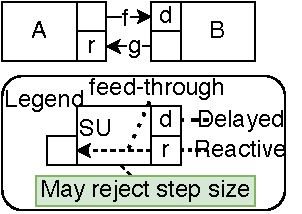
\includegraphics[width=0.5\textwidth]{images/simple_example.pdf}
            \end{figure}
            \begin{figure}
                \centering
                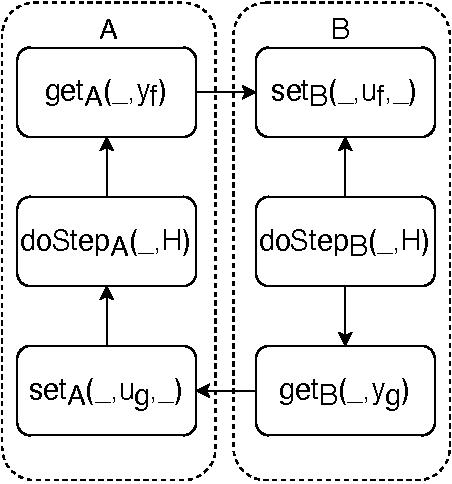
\includegraphics[width=0.55\textwidth]{images/simple_scenario_graph.pdf}
            \end{figure}
    \end{column}%
    \hfill%
    \begin{column}{.48\textwidth}
        \begin{algorithm}[H]
            \caption{Step function of scenario}
            \begin{algorithmic}[1]
              \scriptsize
              \State $\stateafter{A}{s+H} \gets \fdoStep{A}(\stateafter{A}{s}, H)$
              \State $\stateafter{B}{s+H} \gets \fdoStep{B}(\stateafter{B}{s}, H)$
              \State $F_v \gets \fget{B}(\stateafter{B}{s+H}, \outputvar{F})$
              \State $\stateafter{A}{s+H} \gets \fset{A}(\stateafter{a}{s+H}, \inputvar{F}, F_v)$
              \State $x_v \gets \fget{A}(\stateafter{A}{s+H}, \outputvar{x})$
              \State $\stateafter{B}{s} \gets \fset{B}(\stateafter{B}{s+H}, \inputvar{x}, x_v)$
            \end{algorithmic}
          \end{algorithm}
    \end{column}%
    \end{columns}
\end{frame}

\begin{frame}{The currently implemented rules (For reference)}
    \begin{definition}[Step Operation Graph]\label{def:operation_graph}
        Given a co-simulation scenario $\tuple{\fmus, \coupling, \mayReject, \allfeedthroughs, \allreactivity}$, we define the step operation graph where each node represents an operation $\fset{c}(\dontcare, \inputvar{c}, \dontcare)$, $\fdoStep{c}(\dontcare, H)$, or $\fget{c}(\dontcare, \outputvar{c})$, of some fmu $c \in \fmus$, $\outputvar{c} \in \outputs{c}$, and $\inputvar{c} \in \inputs{c}$.
        The edges are created according to the following rules:
        \begin{compactenum}
          \item For each $c \in \fmus$ and $\inputvar{c} \in \inputs{c}$, if $\coupling(\inputvar{c}) = \outputvar{d}$, add an edge $\fget{d}(\dontcare, \outputvar{d}) -> \fset{c}(\dontcare, \inputvar{c}, \dontcare)$;
          \item For each $c \in \fmus$ and $\outputvar{c} \in \outputs{c}$, add an edge $\fdoStep{c}(\dontcare, H) -> \fget{c}(\dontcare, \outputvar{c})$;
          \item For each $c \in \fmus$ and $\inputvar{c} \in \inputs{c}$, if $\reactivity{c}(\inputvar{c})=\true$, add an edge $\fset{c}(\dontcare, \inputvar{c}, \dontcare) -> \fdoStep{c}(\dontcare, H)$;
          \item For each $c \in \fmus$ and $\inputvar{c} \in \inputs{c}$, if $\reactivity{c}(\inputvar{c})=\false$, add an edge $\fdoStep{c}(\dontcare, H) -> \fset{c}(\dontcare, \inputvar{c}, \dontcare)$;
          \item For each $c \in \fmus$ and $(\inputvar{c},\outputvar{c}) \in \feedthrough{c}$, add an edge 
          $\fset{c}(\dontcare, \inputvar{c}, \dontcare) -> \fget{c}(\dontcare, \outputvar{c})$.
        \end{compactenum}
      \end{definition}      
\end{frame}


\begin{frame}{Co-simulation scenarios categories}
    \begin{columns}[T] 
        \begin{column}{.48\textwidth}
        Simple Scenarios:
        \begin{itemize}
            \item The current approach works for these examples!
            \item No Algebraic Loops
            \item Step negotiation \textbf{not} needed!
        \end{itemize}
        \begin{figure}
            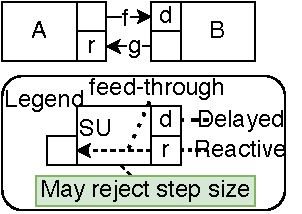
\includegraphics[scale=0.6]{images/simple_example.pdf}
            \end{figure}
        \end{column}%
        \hfill%
        \begin{column}{.48\textwidth}
        Complex Scenarios:
        \begin{itemize}
            \item The standard approach does \textbf{not} work!
            \item Algebraic Loops - a port depends on itself
            \item Step negotiation needed!
        \end{itemize}
        \begin{figure}
            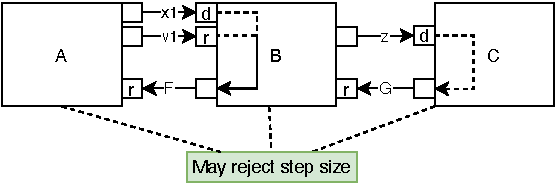
\includegraphics[scale=0.6]{images/loop_within_loop.pdf}
        \end{figure}
        \end{column}%
    \end{columns}
\end{frame}


\section{Complex Scenarios}


\begin{frame}{Simulation of complex scenario}
    \begin{columns}[T]
        \begin{column}{0.5\textwidth}
            \begin{itemize}
                \item Simulated using a correct configuration (Step size + Fixed-points).
                \item An incorrect configuration breaks the preconditions.
                \item Simulation strategy is to use an iterative search to establish a configuration.
                \item The search is restarted after unsuccessful tries (using restore and save).
            \end{itemize}
        \end{column}
        \begin{column}{0.5\textwidth}
            \begin{algorithm}[H]
                \caption{Simulation of complex scenarios.}
            \label{alg:algorithm_step}
            \begin{algorithmic}[1]
              \scriptsize
                \State Save SUs
                \While{$!correctConfiguration$} 
                \State Iterative search
                \State $correctConfiguration \gets isCorrect()$
                \If{$!correctConfiguration$}
                    \State Restore SUs
                \EndIf
                \EndWhile
            \end{algorithmic} 
          \end{algorithm}
        \end{column}
    \end{columns}    
\end{frame}

\begin{frame}{Algebraic Loops}
    \textbf{Happens if}: The value on a ports depends on itself.\\
    \textbf{Example of the two kinds of Algebraic Loops}: 
    \begin{columns}[T] % align columns
        \begin{column}{.48\textwidth}
            \begin{figure}    
                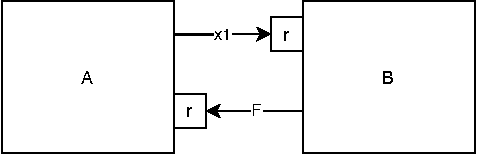
\includegraphics[width=0.9\textwidth]{images/reactive_loop_scenario.pdf}
                \caption{Reactivity Loop}
            \end{figure}
    \end{column}%
    \hfill%
    \begin{column}{.48\textwidth}
        \begin{figure}    
            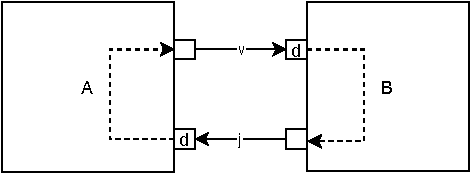
\includegraphics[width=0.9\textwidth]{images/feedthroughloop.pdf}
            \caption{Feed-through Loop}
        \end{figure}
    \end{column}%
    \end{columns}
    \textbf{How do we simulate this}: Fixed-point iteration - The simulation iteratively searches for a fixed-point on all the output ports between two successive iterations.\\
    \textbf{Problem:} Introduces non-trivial SCCs in the graph - no topological order can be found.
\end{frame}

\begin{frame}{Step negotiation}
    \textbf{Happens if}: A scenario contains SUs that may reject to take a step of arbitrary size.\\
    \textbf{Example}: 
    \begin{columns}[T] % align columns
        \begin{column}{.48\textwidth}
            \begin{figure}    
                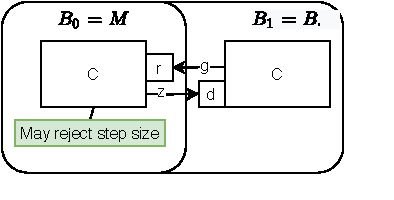
\includegraphics[width=0.9\textwidth]{images/step_scenario.pdf}
            \end{figure}
    \end{column}%
    \hfill%
    \begin{column}{.48\textwidth}
        \begin{figure}    
            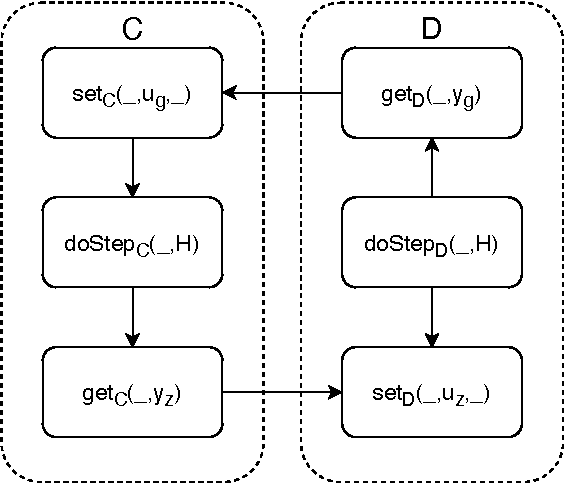
\includegraphics[width=0.7\textwidth]{images/step_scenario_original.pdf}
            \caption{The graph.}
        \end{figure}
    \end{column}%
    \end{columns}
    \textbf{How do we simulate this}: The simulation iteratively searches for a step all SUs are able to perform.
\end{frame}


\begin{frame}{The current state of the two kinds of complex scenarios}
    \begin{columns}[T] 
        \begin{column}{.48\textwidth}
            Algebraic Loops - SCC in graph
            \begin{figure}    
                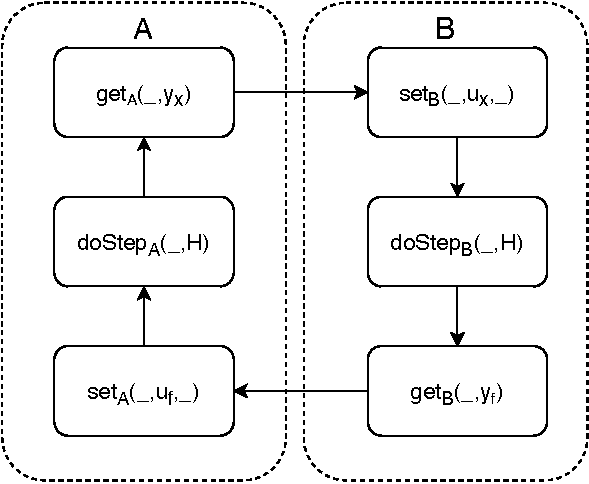
\includegraphics[width=0.9\textwidth]{images/reactive_step_graph.pdf}
            \end{figure}  
        \end{column}
    \hfill%
    \begin{column}{.48\textwidth}
        Step negotiation - no SCC in graph
        \begin{figure}    
            \centering
            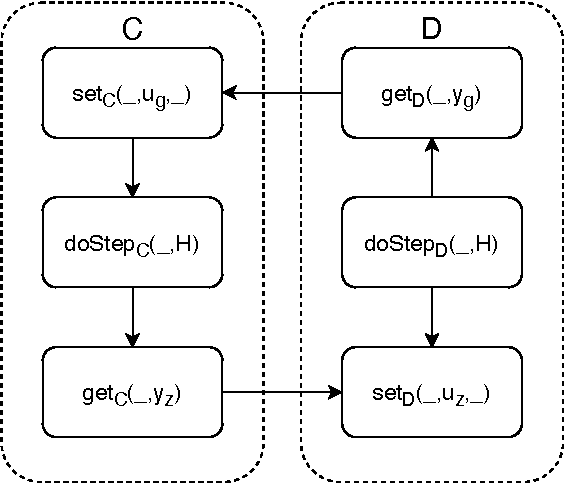
\includegraphics[width=0.9\textwidth]{images/step_scenario_original.pdf}
        \end{figure}
    \end{column}
    \end{columns}
\end{frame}


\begin{frame}{Extending the approach to handle complex scenarios?}
    \begin{block}{What is needed?}
        \begin{enumerate}
            \item A way to identify complex scenarios.
            \begin{itemize}
                \item Step negotiation
                \item Algebraic Loops
                \begin{itemize}
                    \item Reactive loops
                    \item Feed-through loops
                \end{itemize}        
            \end{itemize}
            \item A way to handle complex scenarios
            \begin{itemize}
                \item A method to break non-trivial SCCs - to obtain a topological order.

            \end{itemize}
        \end{enumerate}
    \end{block}
\end{frame}


\begin{frame}{Reactive Loops}
    \textbf{Happens if}: An algebraic loop exist with time-progression.\\
    \textbf{Identifiable:} It is a non-trivial SCC with at least one \textit{Step}-node and no edges between two \textit{Step}-nodes. \\
    \textbf{Example}: 
    \begin{columns}[T] % align columns
        \begin{column}{.48\textwidth}
            \begin{figure}    
                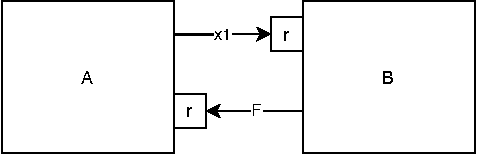
\includegraphics[width=0.9\textwidth]{images/reactive_loop_scenario.pdf}
            \end{figure}
    \end{column}%
    \hfill%
    \begin{column}{.48\textwidth}
        \begin{figure}    
            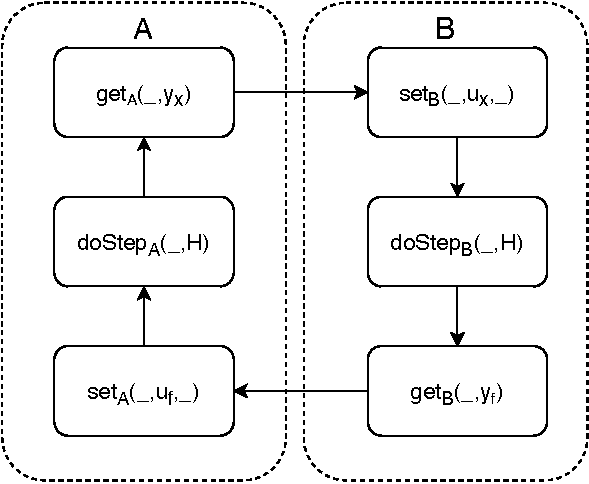
\includegraphics[width=0.9\textwidth]{images/reactive_step_graph.pdf}
        \end{figure}
    \end{column}%
    \end{columns}
\end{frame}

\begin{frame}{Reactive Loop - How to extract a fixed-point procedure?}
    \textbf{Observations}: 
    \begin{itemize}
        \item Progression of time in an iteratively search $\implies$ Restoration of state is needed - to give us more chances to find the fixed-points. 
        \item The convergence criteria are a fixed-point on all output ports.
    \end{itemize}
    \begin{block}{Conclusion}
        We need a way to break a non-trivial SCC!        
    \end{block}
\end{frame}

\begin{frame}{Breaking a non-trivial SCC}
    \begin{block}{Reduction}
        The non-trivial SCC of Algebraic loops are broken by guessing some input values to destroy edges in the graph!

    \end{block}
    Two different kinds of reductions exist:
    \begin{itemize}
        \item Maximum reduction: Provide guesses for all inputs for all SUs - we should use this technique. 
        \item Minimum reduction: Provide a guess for the minimum number of inputs to break the cycle.
    \end{itemize}
    Preferably the user should describe the type of reduction used - this is scenario dependent!
\end{frame}

\begin{frame}{Reduction schemes}
    The SCC is broken using reduction scheme:
    \begin{columns}[T] 
        \begin{column}{.48\textwidth}
            \begin{figure}    
                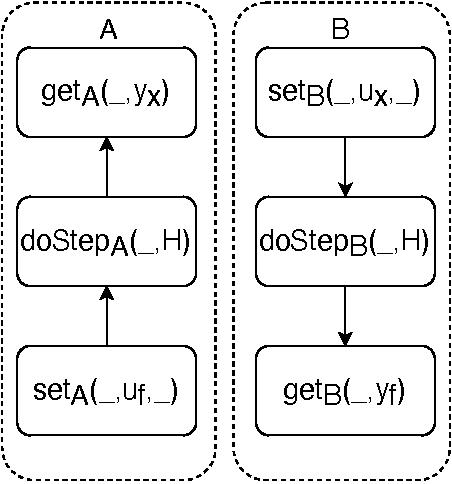
\includegraphics[width=0.8\textwidth]{images/jacobian_reduced_graph.pdf}
                \caption{Maximal reduction.}
            \end{figure}  
        \end{column}
    \hfill%
    \begin{column}{.48\textwidth}
        \begin{figure}    
            \centering
            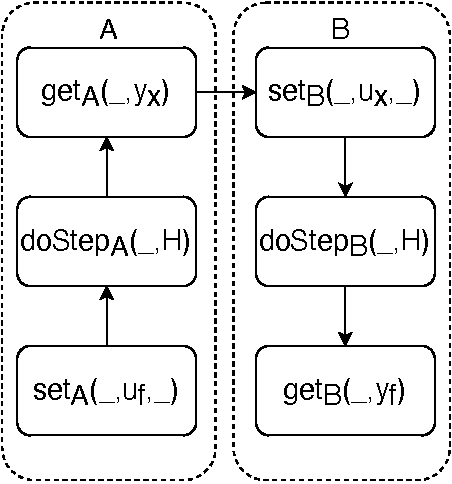
\includegraphics[width=0.8\textwidth]{images/gauss_reduced_graph.pdf}
            \caption{Minimal reduction.}
        \end{figure}
    \end{column}
    \end{columns}
\end{frame}

\begin{frame}{Maximum reduction:}
    \textbf{Technique}: Provide guesses for the for all inputs.
    \begin{columns}[T] % align columns
        \begin{column}{.48\textwidth}
            \begin{figure}    
                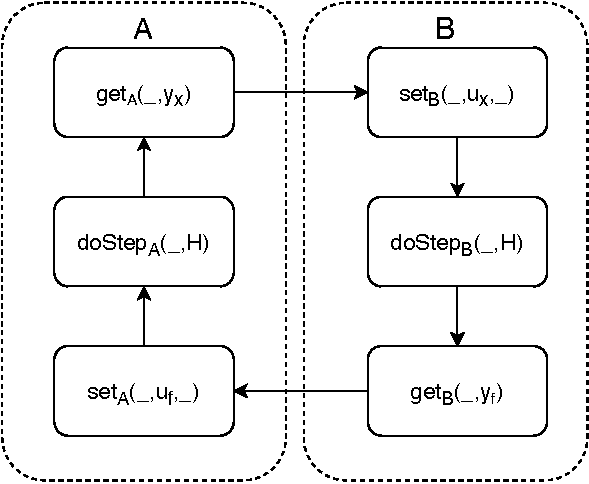
\includegraphics[width=0.8\textwidth]{images/reactive_step_graph.pdf}
                \caption{Original Graph}
            \end{figure}
    \end{column}%
    \hfill%
    \begin{column}{.48\textwidth}
        \begin{figure}    
            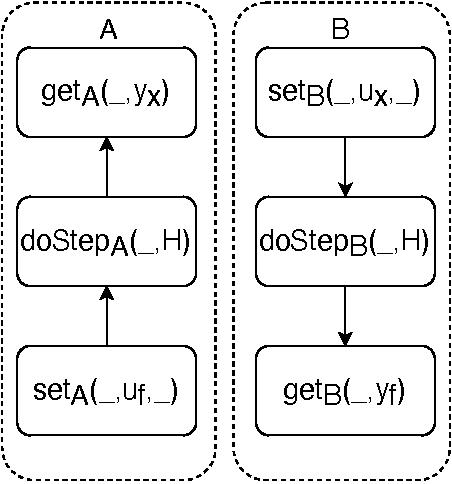
\includegraphics[width=0.7\textwidth]{images/jacobian_reduced_graph.pdf}
            \caption{Maximum Reduction}
        \end{figure}
    \end{column}%
    \end{columns}
    \textbf{Consequence:}
    All edges from \textit{Get}-nodes to reactive \textit{Set}-nodes disappear in reactive loops.
    In feed-through loops, we also remove connections to delayed ports.  
\end{frame}

\begin{frame}{Maximum reduction - obtaining an algorithm:}
    \begin{columns}[T] % align columns
        \begin{column}{.48\textwidth}
            \begin{algorithm}[H]
                \begin{algorithmic}
                  \scriptsize
                  \State Save SUs   
                  \While{$!conv$}
                  \State $\stateafter{A}{s} \gets \fset{A}(\stateafter{A}{s}, \inputvar{j}, j_v)$
                  \State $\stateafter{B}{s} \gets \fset{B}(\stateafter{B}{s}, \inputvar{v}, v_v)$
                  \State $\stateafter{A}{s+h}, \gets \fdoStep{C}(\stateafter{A}{s}, h)$
                  \State $\stateafter{B}{s+h}, \gets \fdoStep{B}(\stateafter{B}{s}, h)$
                  \State $v_a \gets \fget{A}(\stateafter{A}{s+h}, \outputvar{v})$
                  \State $j_a \gets \fget{B}(\stateafter{B}{s+h}, \outputvar{j})$
                  \State $conv \gets CheckCon((j_a, j_v),(v_a, v_v))$
                  \If{$!conv$}
                      \State Restore     
                  \EndIf
                  \State $v_v \gets v_a$
                  \State $j_v \gets j_a$
              \EndWhile
              \end{algorithmic}
              \caption{}
              \end{algorithm}
    \end{column}%
    \hfill%
    \begin{column}{.48\textwidth}
        \begin{figure}    
            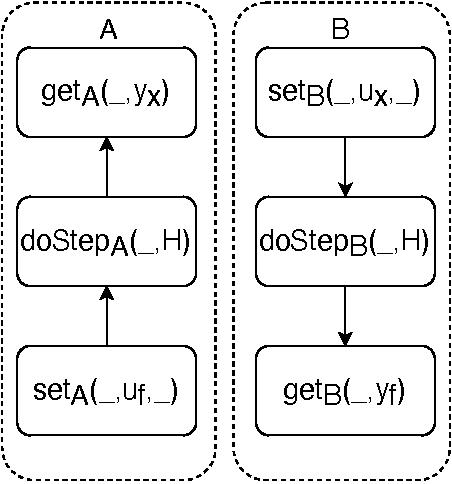
\includegraphics[width=0.8\textwidth]{images/jacobian_reduced_graph.pdf}
            \caption{Maximum Reduction to get an acyclic graph.}
        \end{figure}
    \end{column}%
    \end{columns}    
\end{frame}


\begin{frame}{Feed-through Loops}
    \textbf{Happens if}: A direct dependence of the value on an output port to itself.\\
    \textbf{Identifiable:} It is a non-trivial SCC with no \textit{Step}-nodes. \\
    \textbf{Example}: 
    \begin{columns}[T] % align columns
        \begin{column}{.48\textwidth}
            \begin{figure}    
                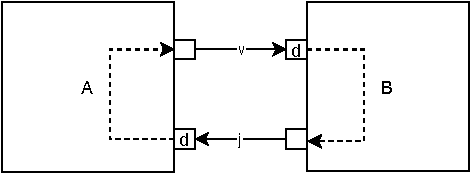
\includegraphics[width=0.9\textwidth]{images/feedthroughloop.pdf}
            \end{figure}
    \end{column}%
    \hfill%
    \begin{column}{.48\textwidth}
        \begin{figure}    
            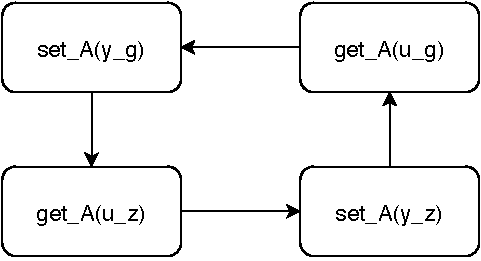
\includegraphics[width=0.9\textwidth]{images/feed_loop_dep.pdf}
        \end{figure}
    \end{column}%
    \end{columns}
\end{frame}

\begin{frame}{Solving Feed-through Loops:}
    \textbf{Observations}: 
    \begin{itemize}
        \item No progression of time in an iteratively search $\implies$ Restoration of state is \textbf{not} needed.
        \item Thus no need for \textit{Restore} and \textit{Save}.
    \end{itemize}
    \begin{block}{Conclusion}
        The graph is made acyclic using reductions - similarly to the reactive loops! \\
        The algorithm is found from the acyclic graph.
    \end{block}
\end{frame}

\begin{frame}{Strategy in Maude for Algebraic Loops}
    \begin{enumerate}
        \item Detection If SCC in graph we should detect its nature
        \begin{itemize}
            \item Feed-through - no time progression
            \item Reactive Loop - time progression (need state restoration)
        \end{itemize}
        \item Mark as special loop-action with convergence criteria and restore-actions
        \item Remove edges (Reduction scheme) 
        \item Extract actions of loop body (hopefully using normal rules).
    \end{enumerate}  
    \emph{We should be careful that not all actions end up inside the loop-action}
\end{frame}


\begin{frame}{Synthesizing Complex Scenarios - Step negotiation}
    The trick here is to highlight that step negotiation - we can easily calculate the SUs $(B)$ that should be part of the step negotiation, iteratively until we reach a fixed point.
    \begin{columns}[T] 
        \begin{column}{.48\textwidth}
            \begin{figure}    
                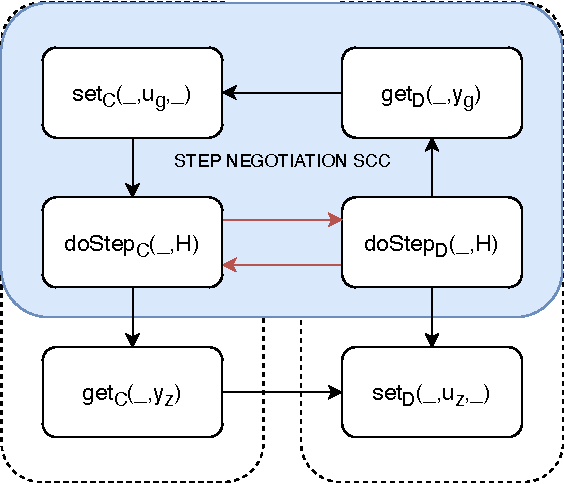
\includegraphics[width=0.8\textwidth]{images/step_scenario_graph.pdf}
                \caption{Step graph - the blue part shows the iterative search.}
            \end{figure}  
        \end{column}
    \hfill%
    \begin{column}{.48\textwidth}
        \begin{algorithm}[H]
            \caption{Step negotiation.}
        \begin{algorithmic}[1]
          \scriptsize
            \While{$!\stepfound$} 
            \State $(\stateafter{D}{s+h_D},h_D) \gets \fdoStep{D}(\stateafter{D}{s}, h)$
            \State $g_v \gets \fget{D}(\stateafter{D}{s+h_D}, \outputvar{g})$       
            \State $\stateafter{C}{s} \gets \fset{C}(\stateafter{C}{s}, \inputvar{G}, G_v)$
            \State $(\stateafter{C}{s+h_C},h_C) \gets \fdoStep{C}(\stateafter{C}{s}, h_D)$
            \State $h \gets min(h_C, h_D)$
            \State $\stepfound \gets h == h_C \land h == h_D$
            \If{$!\stepfound$}
                \State Restore SUs
            \EndIf
            \EndWhile
        \end{algorithmic} 
      \end{algorithm}
    \end{column}
    \end{columns}
\end{frame}

\begin{frame}{Step negotiation}
    The iterative search for a step all SUs can take!\\
    \textbf{Observations}: 
    \begin{itemize}
            \item If one SU rejects a step of size $H$, all SUs that has taken a step of $H$ should be backtracked.
            \item We want to \emph{limit the number of SUs} ($B$) that need to be backtracked.
            \item Step negotiation should be performed first in a simulation step.
            % \item \textbf{Consist of:} All actions performed before a $\fdoStep{\dontcare}$ that may fail.
            % \begin{itemize}
            %     \item Transitive reactive connections to an SU that can reject a step.
            % \end{itemize}
    \end{itemize}
    \begin{block}{Calculating $B$ - The set of SUs that should be backtracked}
        Iterative calculated by including all SUs reactive coupled to an SU in $B$ until one reaches a fixed-point.
    \end{block}
    \begin{figure}    
        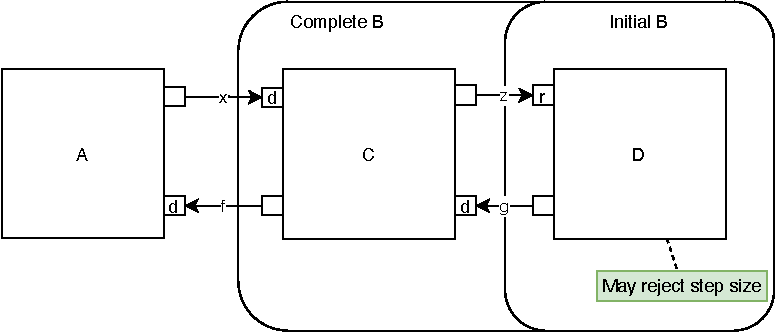
\includegraphics[width=0.6\textwidth]{images/calcB.pdf}
    \end{figure} 
\end{frame}


\begin{frame}{Highlighting the Step negotiation in the graph}
    \begin{alertblock}{Adding edges to introduce a non-trivial SCC}
        \begin{itemize}
            \item Add edges between the \textit{doStep}-nodes of $c$ and $d$ where $c,d \in B$. 
        \end{itemize}
    \end{alertblock}
    \begin{block}{Making the step negotation the intial object}
        \begin{itemize}
            \item Adding edges from all $doStep$ of $c \in B$ to all $doStep$ of $d \notin B$.
            \begin{itemize}
                \item This adds no new non-trivial SCC.
            \end{itemize}
        \end{itemize} 
    \end{block}
    \begin{figure}[H]
        \centering
        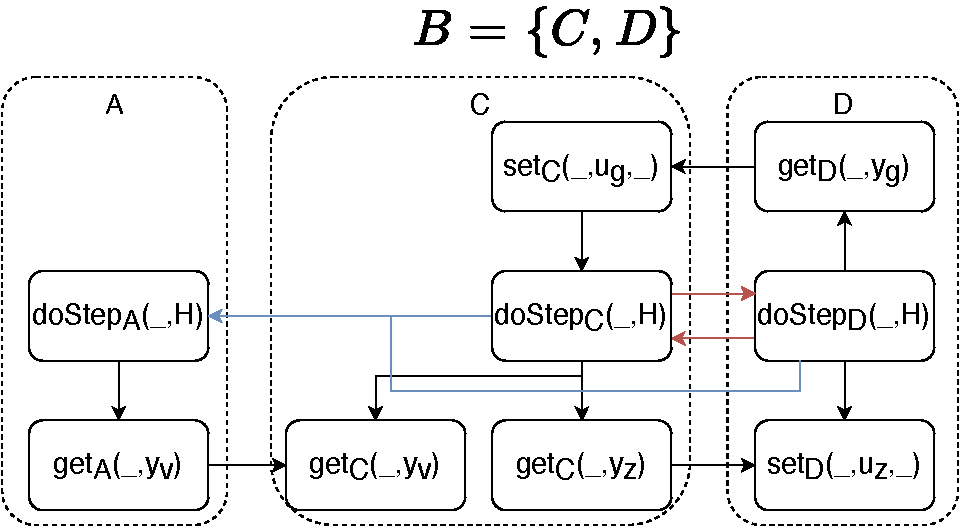
\includegraphics[width=0.65\textwidth]{images/step_scenario_graph_extended.pdf}
      \end{figure}
\end{frame}

\begin{frame}{Step negotiation SCCs to an algorithm}
    \textbf{Identifiable:} A non-trivial SCC with \textit{Step}-nodes and direct edges between two \textit{Step}-nodes.\\
    \textbf{Strategy:} Remove the edges between the $B$-nodes - and use the topological order.
    \begin{columns}[T] % align columns
        \begin{column}{.48\textwidth}
            \begin{figure}    
                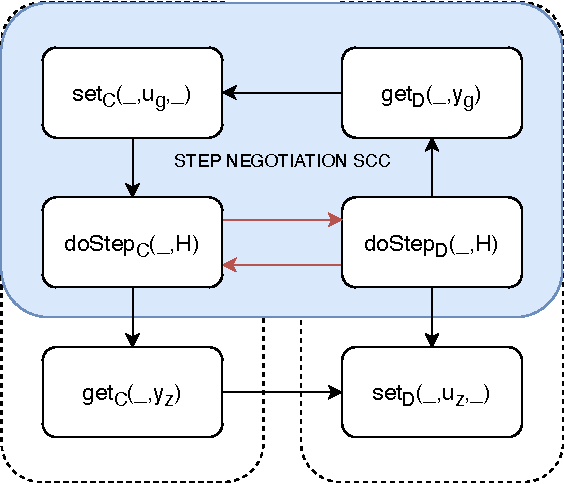
\includegraphics[width=0.95\textwidth]{images/step_scenario_graph.pdf}
            \end{figure}
    \end{column}%
    \hfill%
    \begin{column}{.48\textwidth}
        \begin{algorithm}[H]
        \caption{Step negotiation.}
        \begin{algorithmic}[1]
            \scriptsize
            \While{$!step\_found$}
            \State $\stateafter{D}{s+h_D} \gets \fdoStep{D}(\stateafter{D}{s}, h)$
            \State $g_v \gets \fget{D}(\stateafter{D}{s+h_D}, \outputvar{g})$       
            \State $\stateafter{C}{s} \gets \fset{C}(\stateafter{C}{s}, \inputvar{G}, G_v)$
            \State $\stateafter{C}{s+h_C} \gets \fdoStep{C}(\stateafter{C}{s}, h_D)$
            \State $h \gets min(h_C, h_D)$
            \State $step\_found \gets h == h_C \land h == h_D$
            \If{$!step\_found$}
                \State Restore SUs in $B$
            \EndIf
            \EndWhile
            \State Rest of Simulation
        \end{algorithmic}
        \end{algorithm}
    \end{column}%
    \end{columns}
\end{frame}

\begin{frame}{Strategy in Maude for Step Negotiation}
    \begin{columns}[T] 
        \begin{column}{.48\textwidth}
            \begin{enumerate}
                \item Mark the SUs that may reject a step - a part of the scenario.
                \item Calculate the set B - initially.
                \item If B is non-empty
                \begin{itemize}
                    \item Save SUs in B
                \end{itemize}
                \item Mark as special step-loop-action with convergence criteria and restore-actions
                \item Extract actions for loop body (hopefully using normal rules).
            \end{enumerate}  
        \end{column}
    \hfill%
        \begin{column}{.48\textwidth}
            \begin{figure}    
                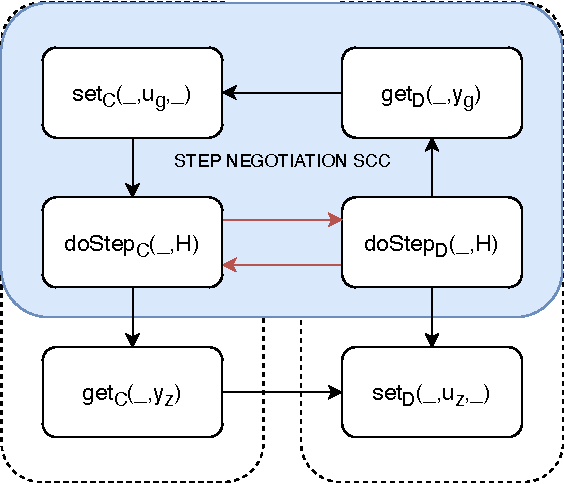
\includegraphics[width=0.8\textwidth]{images/step_scenario_graph.pdf}
                \caption{The graph - the blue part shows should be in the iterative search.}
            \end{figure}  
        \end{column}
    \end{columns}
    \emph{Again we should be careful that not all actions end up inside the step-loop-action}
\end{frame}

\begin{frame}{Scenario subject to step negotiation and algebraic loops}
    The approach also works for nested complex scenarios.
    \begin{enumerate}
        \item Handle the step negotiation.
        \item Handle the algebraic loops inside.
    \end{enumerate}

    \begin{figure}    
        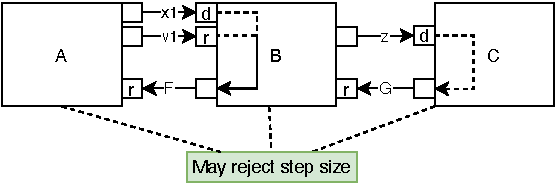
\includegraphics[width=0.5\textwidth]{images/loop_within_loop.pdf}
    \end{figure}
    \begin{figure}   
        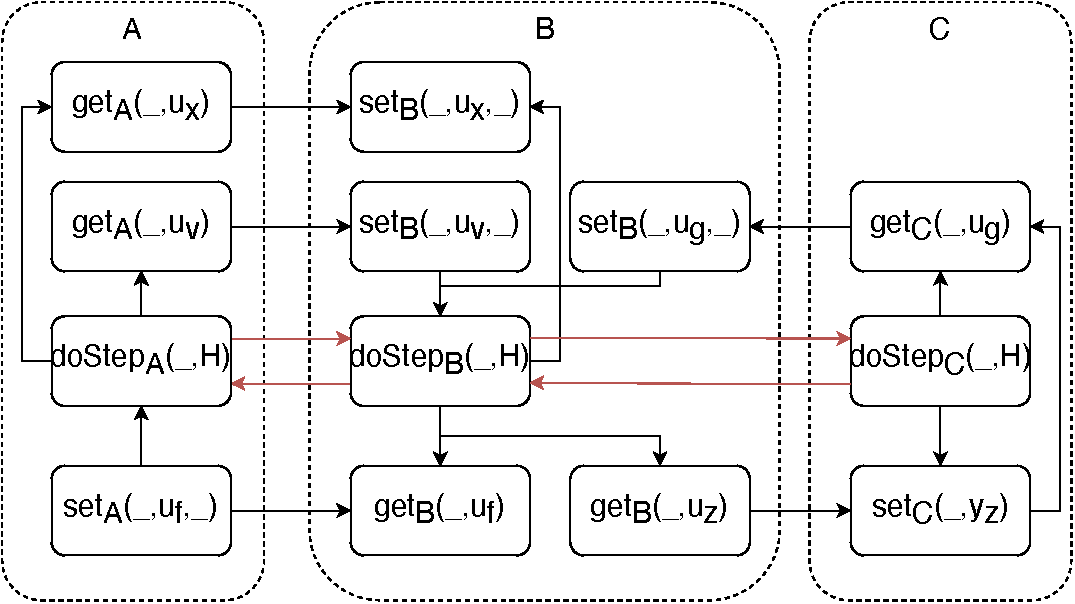
\includegraphics[width=0.5\textwidth]{images/nested_graph.pdf}
    \end{figure}
\end{frame}

\begin{frame}{Next steps}
    \begin{enumerate}
        \item Implementation of step negotiation.
        \item Implementation of algebraic loops.
        \item Logging of the algorithm to the global state - so one can inspect the resulting algorithm.
        \item Implementation of nested complex scenarios.
        \begin{itemize}
            \item Subject to both step negotiation and algebraic loops.
        \end{itemize}
        \item Adaptive co-simulation (changing input configurations).
    \end{enumerate}  
\end{frame}


\end{document}